% The three levels of DRC in a 2.5D assembly.
% Levels 1 and 2 are ordinary PDK DRC. Level 3 is the one the ADK ships.
% Deliberately the same layout as tikz_verification_levels, so the two axes of
% assembly verification can be read against each other.
\documentclass[border=4pt]{standalone}
\usepackage{tikz}
\usetikzlibrary{arrows.meta, positioning, calc, fit}
\usepackage[T1]{fontenc}
\usepackage{lmodern}

% Hyphen breaks inside the small figure labels read badly.
\hyphenpenalty=10000
\exhyphenpenalty=10000

\definecolor{IHPfg}{RGB}{0,80,139}
\definecolor{IHPaccent}{RGB}{109,112,114}
\definecolor{IHPgreen}{RGB}{65,155,75}

\begin{document}
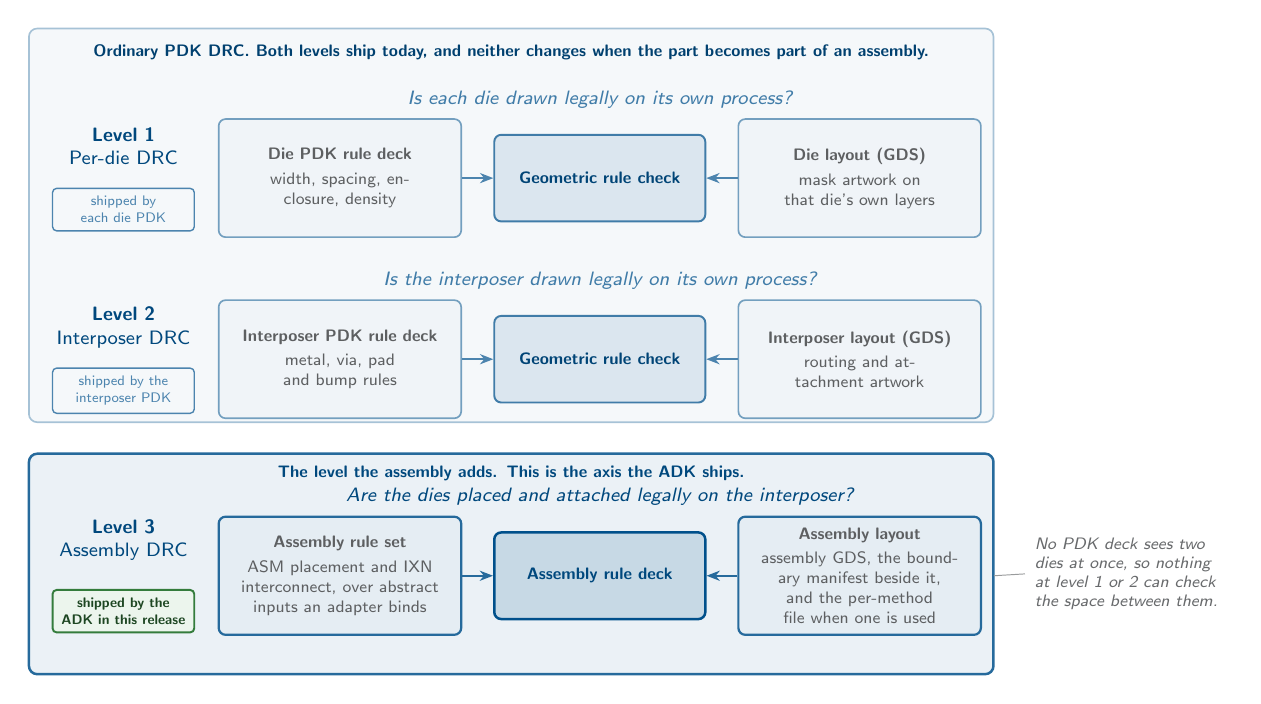
\begin{tikzpicture}[
    x=1mm, y=1mm,
    >=Stealth,
    adkside/.style={
        rectangle, rounded corners=2.5pt,
        draw=IHPfg!55, fill=IHPfg!6, line width=0.6pt,
        text width=28mm, minimum height=15mm,
        font=\sffamily\fontsize{6}{7.2}\selectfont, text=IHPaccent!85!black,
        align=center, inner sep=1.4mm
    },
    adkcomp/.style={
        rectangle, rounded corners=2.5pt,
        draw=IHPfg!75, fill=IHPfg!14, line width=0.7pt,
        text width=24mm, minimum height=11mm,
        font=\sffamily\fontsize{6.2}{7.4}\selectfont\bfseries, text=IHPfg!85!black,
        align=center, inner sep=1.4mm
    },
    adksidelive/.style={
        rectangle, rounded corners=2.5pt,
        draw=IHPfg!85, fill=IHPfg!10, line width=0.8pt,
        text width=28mm, minimum height=15mm,
        font=\sffamily\fontsize{6}{7.2}\selectfont, text=IHPaccent!85!black,
        align=center, inner sep=1.4mm
    },
    adkcomplive/.style={
        rectangle, rounded corners=2.5pt,
        draw=IHPfg, fill=IHPfg!22, line width=0.9pt,
        text width=24mm, minimum height=11mm,
        font=\sffamily\fontsize{6.2}{7.4}\selectfont\bfseries, text=IHPfg!90!black,
        align=center, inner sep=1.4mm
    },
    adklevel/.style={
        text width=19mm, align=center,
        font=\sffamily\fontsize{7}{8.4}\selectfont, text=#1
    },
    adkbadge/.style={
        rectangle, rounded corners=1.5pt,
        draw=#1, line width=0.5pt,
        text width=16mm, align=center, inner sep=1mm,
        font=\sffamily\fontsize{5.2}{6.2}\selectfont, text=#1
    },
    adkbadgeship/.style={
        rectangle, rounded corners=1.5pt,
        draw=IHPgreen!80!black, fill=IHPgreen!10, line width=0.7pt,
        text width=16mm, align=center, inner sep=1mm,
        font=\sffamily\fontsize{5.2}{6.2}\selectfont\bfseries, text=IHPgreen!45!black
    },
    adkask/.style={
        font=\sffamily\fontsize{6.6}{8}\selectfont\itshape, text=#1, align=center
    },
    adkgroup/.style={
        text width=110mm, align=center,
        font=\sffamily\fontsize{6.2}{7.4}\selectfont\bfseries, text=#1
    },
    adkarrow/.style={
        -{Stealth[length=1.7mm, width=1.3mm]}, line width=0.6pt, color=#1
    },
    adknote/.style={
        text width=24mm, align=left,
        font=\sffamily\fontsize{5.6}{6.8}\selectfont\itshape, text=IHPaccent!95!black
    }
]

% ===== Group A backdrop: the two levels that are ordinary PDK DRC =====
\fill[IHPfg!4, rounded corners=3pt] (-2.5,9) rectangle (120,-41);
\draw[IHPfg!35, line width=0.6pt, rounded corners=3pt] (-2.5,9) rectangle (120,-41);

\node[adkgroup=IHPfg!80!black] at (58.75, 6)
    {Ordinary PDK DRC. Both levels ship today, and neither changes when the part
     becomes part of an assembly.};

% ===== Group B backdrop: the level the assembly adds =====
\fill[IHPfg!8, rounded corners=3pt] (-2.5,-45) rectangle (120,-73);
\draw[IHPfg!85, line width=0.9pt, rounded corners=3pt] (-2.5,-45) rectangle (120,-73);

\node[adkgroup=IHPfg!90!black] at (58.75, -47.5)
    {The level the assembly adds. This is the axis the ADK ships.};

% ===== Level 1: per-die DRC =====
\node[adkask=IHPfg!75] at (70, 0) {Is each die drawn legally on its own process?};

\node[adklevel=IHPfg!90!black] at (9.5, -6)
    {\textbf{Level 1}\\Per-die DRC};
\node[adkbadge=IHPfg!70] at (9.5, -14) {shipped by each die PDK};

\node[adkside] (r1) at (37, -10)
    {\textbf{Die PDK rule deck}\\[0.6mm]width, spacing, enclosure, density};
\node[adkcomp] (c1) at (70, -10) {Geometric rule check};
\node[adkside] (i1) at (103, -10)
    {\textbf{Die layout (GDS)}\\[0.6mm]mask artwork on that die's own layers};

\draw[adkarrow=IHPfg!70] (r1.east) -- (c1.west);
\draw[adkarrow=IHPfg!70] (i1.west) -- (c1.east);

% ===== Level 2: interposer DRC =====
\node[adkask=IHPfg!75] at (70, -23) {Is the interposer drawn legally on its own process?};

\node[adklevel=IHPfg!90!black] at (9.5, -29)
    {\textbf{Level 2}\\Interposer DRC};
\node[adkbadge=IHPfg!70] at (9.5, -37) {shipped by the interposer PDK};

\node[adkside] (r2) at (37, -33)
    {\textbf{Interposer PDK rule deck}\\[0.6mm]metal, via, pad and bump rules};
\node[adkcomp] (c2) at (70, -33) {Geometric rule check};
\node[adkside] (i2) at (103, -33)
    {\textbf{Interposer layout (GDS)}\\[0.6mm]routing and attachment artwork};

\draw[adkarrow=IHPfg!70] (r2.east) -- (c2.west);
\draw[adkarrow=IHPfg!70] (i2.west) -- (c2.east);

% ===== Level 3: assembly DRC, the shipped axis =====
\node[adkask=IHPfg!90!black] at (70, -50.5)
    {Are the dies placed and attached legally on the interposer?};

\node[adklevel=IHPfg!90!black] at (9.5, -56)
    {\textbf{Level 3}\\Assembly DRC};
\node[adkbadgeship] at (9.5, -65) {shipped by the ADK in this release};

\node[adksidelive] (r3) at (37, -60.5)
    {\textbf{Assembly rule set}\\[0.6mm]ASM placement and IXN interconnect, over abstract inputs an adapter binds};
\node[adkcomplive] (c3) at (70, -60.5) {Assembly rule deck};
\node[adksidelive] (i3) at (103, -60.5)
    {\textbf{Assembly layout}\\[0.6mm]assembly GDS, the boundary manifest beside it, and the per-method file when one is used};

\draw[adkarrow=IHPfg!85] (r3.east) -- (c3.west);
\draw[adkarrow=IHPfg!85] (i3.west) -- (c3.east);

% Callout on why no PDK deck can reach this level
\node[adknote, anchor=north west] (note) at (124, -54.5)
    {No PDK deck sees two dies at once, so nothing at level 1 or 2 can check
     the space between them.};

\draw[IHPaccent!70, line width=0.35pt] (note.west) -- ([xshift=1.5mm]i3.east);

\end{tikzpicture}
\end{document}
